%!TEX root = dolgozat.tex
%%%%%%%%%%%%%%%%%%%%%%%%%%%%%%%%%%%%%%%%%%%%%%%%%%%%%%%%%%%%%%%%%%%%%%%
\chapter{Road signs}\label{ch:SIGNS}
%%%%%%%%%%%%%%%%%%%%%%%%%%%%%%%%%%%%%%%%%%%%%%%%%%%%%%%%%%%%%%%%%%%%%%%

\section{What are road signs}\label{sec:SIGNS:whatAreThey}

Traffic signs control the flow of traffic, worn the driver of hazards ahead, guide the driver to their destination, and inform them of roadway services. There are three basic types of traffic signs all with different shapes: 

- signs that give orders, circular

- warning signs, triangular

- signs that give information, rectangular

The stop sign is an exception,it is an octagon.


A further guide to the function of a sign is its colour. The colors used are red, white, black, and blue. %All triangular signs are red.

Most of the road signs are composed of two parts: a solid band on the outside and the inside figure or number. The inside symbol is usually black. 

\section{Charateristics}\label{sec:SIGNS:character}

\section{Data set}\label{sec:SIGNS:dataSet}

\subsection{Training data}

I used ... . It contains 1213 training images, their size varies from 16x16 to 128x128 pixels, they appear in every perspective and under every lighting condition. The images are divided in 43 categories based on the containd traffic signs.

Altough there is a large amount of training images, they are not devided equally among categories. This                       makes it difficult for the network to learn the specifics of the classes that contain small amounts of images.

I try to equalize the number of training images by generating more images into that category. The original training set contains images that completely contain the traffic sign. Since my purpose is to recognise partially visible road signs too, I generate new images from the old ones by cutting out 70-80\% of them.

\begin{figure}
\centering


\includegraphics{trainingImage}
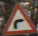
\includegraphics{trainingImage2}
\caption{Example of the training images}

\label{fig:trainingImage}
\end{figure}

\subsection{Test data}

There are 900 test images, containing zero to six traffic signs. They are significantly larger pictures: 1360 x 800 pixels.

\begin{figure}
\centering

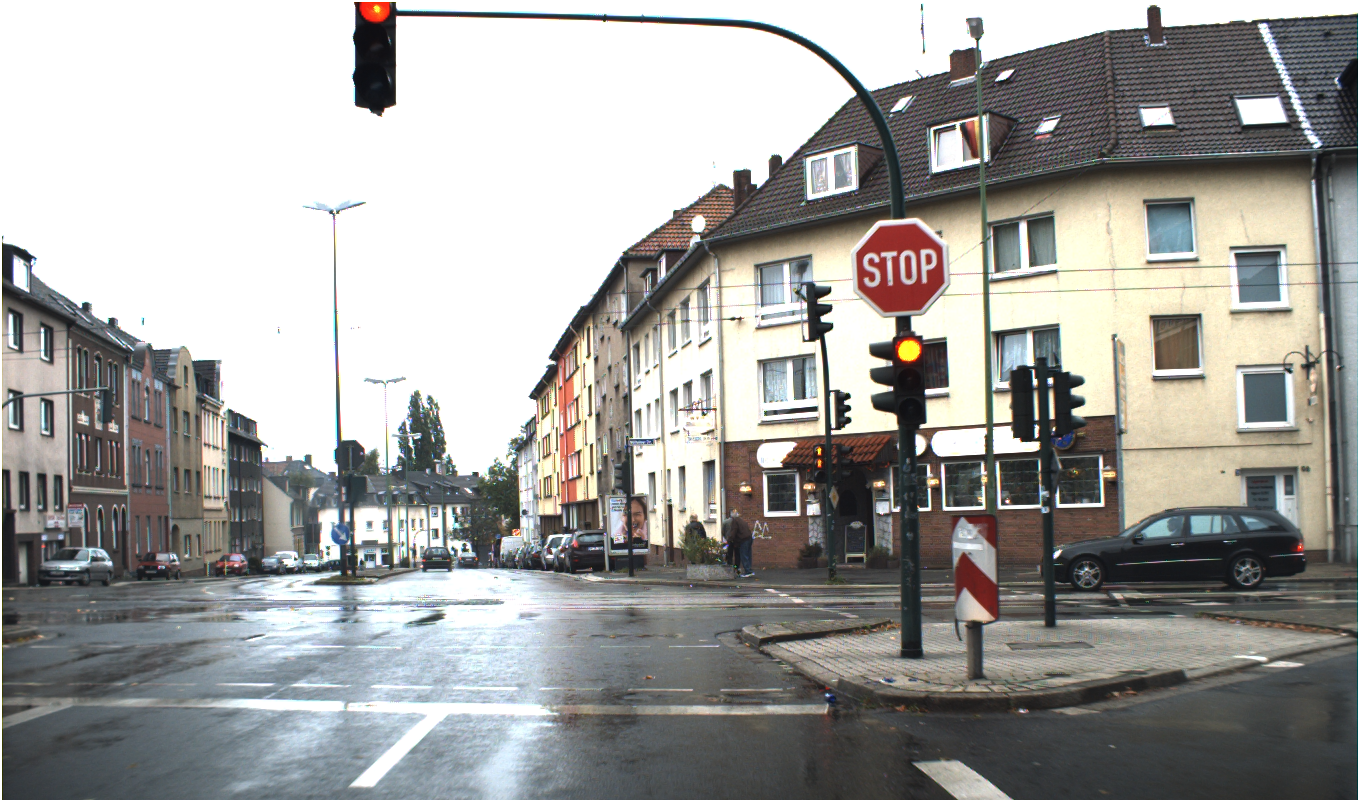
\includegraphics[scale=0.4]{testImage}
\caption{Example of the test images}

\label{fig:trainingImage}
\end{figure}

